\documentclass[a4paper,UTF8]{article}
\usepackage{CJKutf8}
\usepackage[margin=1.25in]{geometry}
\usepackage{color}
\usepackage{graphicx}
\usepackage{amssymb}
\usepackage{amsmath}
\usepackage{amsthm}
\usepackage{multirow}
\usepackage{pdfpages}
\usepackage{tikz}
\usepackage{listings}
\usepackage{xcolor} 
\usepackage{longtable}
\usetikzlibrary{arrows,automata} 

%\setmainfont                    [Ligatures=TeX]{Times New Roman}
\theoremstyle{definition}
\newtheorem*{solution}{Solution}
\newtheorem*{prove}{Proof}

\lstset{
	numbers=left, 
	numberstyle=\tiny,
	frame=shadowbox, 
	breaklines=true, 
	showspaces=false,
 	keywordstyle=\color{purple}\bfseries,
	%identifierstyle=\color{brown!80!black},
 	commentstyle=\color{gray}
	stringstyle=\color{brown!60!black},
	rulesepcolor=\color{red!20!green!20!blue!20}
}
\begin{document}
\begin{CJK}{UTF8}{gkai}
\title{MPLab1-实验报告}
\author{
    \begin{minipage}[b]{0.3\linewidth}
      \begin{flushright}
        Name: 傅小龙\\%\rule{3cm}{0.4pt}\\
        \vbox to 1mm{}
        Grade: 3%\rule{3cm}{0.4pt}
      \end{flushright}
    \end{minipage}
    \hfill
    \begin{minipage}[b]{0.3\linewidth}
      \begin{flushright}
        Dept: CS\\%\rule{3cm}{0.4pt}\\
        \vbox to 1mm{}
        ID: 191220029%\rule{3cm}{0.4pt}
      \end{flushright}
    \end{minipage}
}
\date{}
\maketitle


\begin{CJK*}{UTF8}{gbsn}
\section*{实验目标}
\end{CJK*}
\par 完成单机伪分布式Hadoop系统的安装,运行Hadoop自带的WordCount程序测试。
\begin{CJK*}{UTF8}{gbsn}
\section*{实验过程}
\end{CJK*}
\begin{enumerate}
	\item[1.] 单机操作系统安装\\
	\par 在VMware中创建Linux(Ubuntu 20.02 2)虚拟机.
	\item[2.] 安装SSH\\
	\par 步骤1中创建的虚拟机已经安装有SSH.
	\item[3.] 安装JAVA\\
	\par jdk1.8.0\_321
	\item[4.] 创建用户
	\par 添加hadoop-user用户组,组成员用户myhadoop.\\
	\item[5.] 解压安装Hadoop
	\par 安装的Hadoop版本为2.7.1
	\item[6.] 配置环境变量
\begin{lstlisting}[escapeinside=``]
PATH=$PATH:$HOME/bin 
export JAVA_HOME=/usr/jdk1.8.0_321
export HADOOP_HOME=/home/myhadoop/hadoop-2.7.1 
export PATH=$JAVA_HOME/bin:$HADOOP_HOME/bin:$PATH 
export CLASSPATH=$JAVA_HOME/lib:.
\end{lstlisting}
	\item[7.] 免密码SSH访问配置
	\par 生成SSH认证文件并将秘钥复制到~/.ssh/authorized\_keys文件中。测试登陆结果见Figure1.
	\begin{figure}[h]
    \centering
    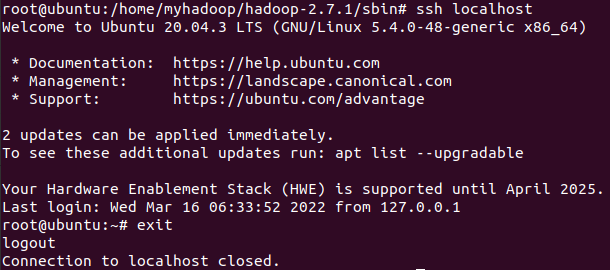
\includegraphics{./ssh.png}
    \caption{SSH访问配置}
    \end{figure} 
	
	\item[8.] 修改Hadoop配置文件
	\par 具体过程参考教材《深入理解大数据》2.2.5节配置Hadoop环境.
	\item[9.] 格式化NameNode
	执行结果见Figure2.
	\begin{figure}[h]
    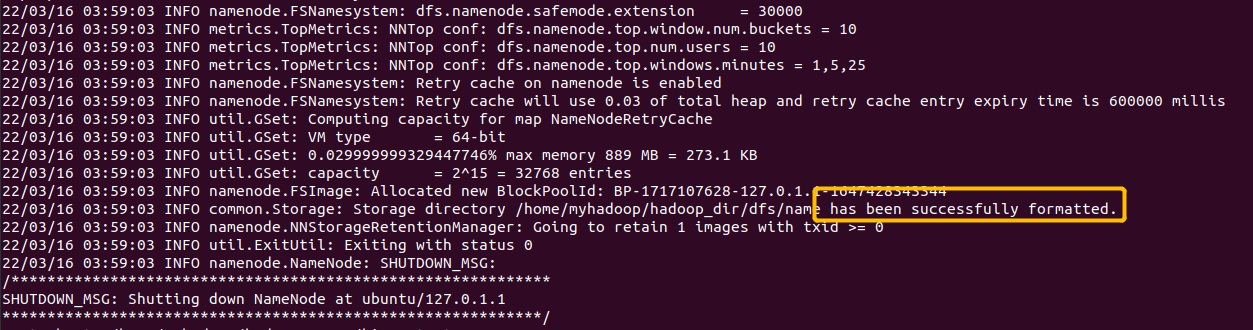
\includegraphics[scale=0.65]{./namenode-format.png}
    \caption{格式化NameNode}
    \end{figure} 

	\item[10.] 启动HDFD和MapReduce
	\par 执行start-all.sh后用jps指令查看进程信息,结果见Figure3.
	\begin{figure}[h]
    \centering
    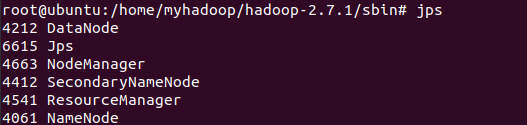
\includegraphics{./start-all-jps.png}
    \caption{jps}
    \end{figure} 
	\item[11.] 停止HDFD和MapReduce
	\par 执行stop-all.sh
	\item[12.] 运行WordCount测试
	\par 重新执行步骤10.\\
		用以下网页
		\begin{enumerate}
		\item[a.] https://github.com/malware-dev/MDK-SE
		\item[b.] https://github.com/malware-dev/MDK-SE/wiki
		\item[c.] https://github.com/malware-dev/MDK-SE/wiki/Api-Index
		\end{enumerate}
		作为输入数据进行词频统计。malware-dev/MDK-SE是github上的一个开源项目,旨在介绍太空工程师可编程模块中提供的C\#接口。用到的这三个页面分别是项目主页、wiki手册主页以及手册中的API目录页面。
	\par 在dfs系统下新建lab1文件夹,然后将测试数据拷贝到该文件夹下的testfile文件夹内.以lab1/out作为输出文件夹,提交任务(见Figure4):
	\begin{figure}[h]
    \centering
    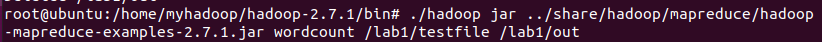
\includegraphics{./submit.png}
    \caption{}
    \end{figure} 
	\par 运行结束后Hadoop Web作业状态查看界面见Figure5:
	\begin{figure}[h!]
    \centering
    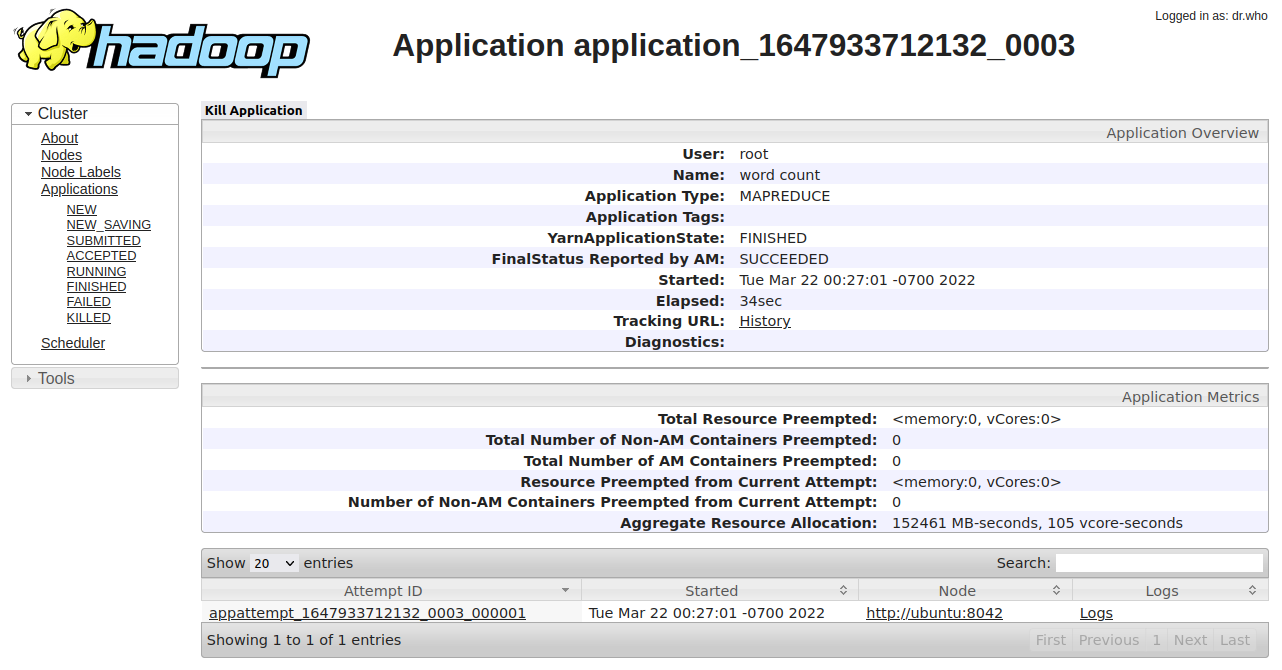
\includegraphics[scale=0.35]{./application.png}
    \caption{作业状态}
    \end{figure} 
	\par 实验输出结果开头部分见Figure6:
	\begin{figure}[h]
    \centering
    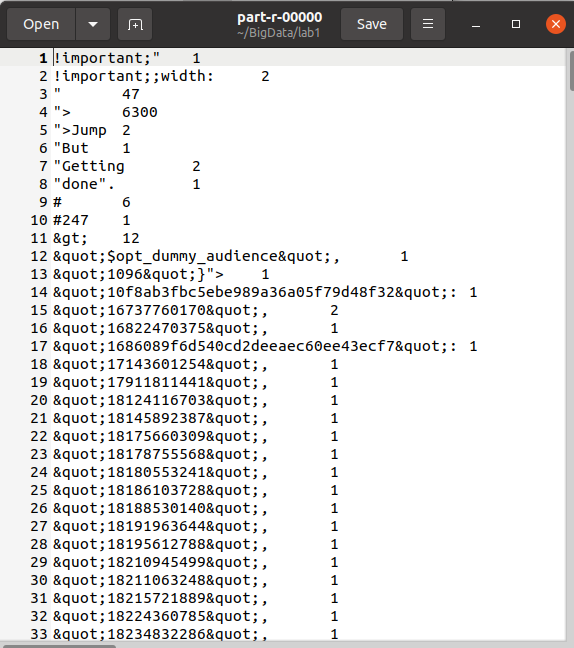
\includegraphics{./out.png}
    \caption{输出结果的开头部分}
    \end{figure} 
\end{enumerate}
\begin{CJK*}{UTF8}{gbsn}
\section*{实验体会}
\end{CJK*}
\par 本次实验中完成了Hadoop单机伪分布式系统的安装。Hadoop系统的安装过程中需要编辑大量的配置文件,这对用户不太友好,是否可以用脚本或设计一个UI界面来引导用户逐步完成Hadoop系统的配置来实现这一步呢?
\par 在实验过程中主要遇到的问题为安装教程可能已经落后于要用到的版本: 2.7.1版本的Hadoop配置文件中并没有mapred-site.xml,而是mapred-site.xml.template,需要将改文件去除.template后缀才能使配置生效。在Web端查看提交作业的状态需要额外配置yarn. 具体过程为在mapred-site.xml中添加如下部分:
\begin{lstlisting}[escapeinside=``]
<property>
	<name>mapreduce.framework.name</name>
	<value>yarn</value>
</property>
\end{lstlisting}
在yarn-site.xml中添加如下部分:
\begin{lstlisting}[escapeinside=``]
<property>
	<name>yarn.nodemanager.aux-services</name>
	<value>mapreduce_shuffle</value>
</property>
\end{lstlisting}
	\par 本次实验中另外遇到的一个问题是在执行任务时进度卡在reduce 0\%阶段。在网上查找原因后发现是虚拟机分配的内存太小。将虚拟机内存扩大后再次执行任务,成功完成。
\end{CJK}
\end{document}
